\chapter{Biology Literature Review}
\label{chp:AnatomyLit}
This chapter aims to describe the biological context within which the project is undertaken. An overview will be given about the anatomy of the ear which is relevant to this study. After which, background will be given about the physiology of each of the five medical signs.

\section{Ear Anatomy} %----------------------------------------------------------------------------------
The area that is available for the Ear-Monitor to make the medical sign measurements is the external ear. It includes the auricle, ear canal with surrounding tissue and the lateral side of the tympanum.  Each part of the ear anatomy will be discussed, especially with regards to its ability to emit information about medical signs or to support the device in another way.

\subsection{Auricle}
The auricle is the visible part of the ear. It forms a C-shaped funnel that protrudes from the scull. Its structure is predominantly formed by yellow elastic cartilage covered in skin. Its complex folded shape differs from person to person, but certain structures are present in all normal auricles and have been named. As can be seen on Figure~\ref{fig:Auricle} the concha is the indented part next to the ear canal. This area is an ideal location for a wearable device. The device can be held in place by the tragus and a probe can easily extend into the ear canal.

\medskip

The external ear is supplied with blood from the auricular arteries. These arteries branch from the carotid artery which supplies the rest of the brain with blood. Being made mostly of cartilage and being at an extremity of the body, the auricle is not a suitable location for taking temperature measurements for its temperature is easily influenced by the ambient conditions.

\medskip

\begin{figure}[h]
\centering
\graphicspath{{figs/}}
\def\svgwidth{200pt}
\input{figs/Auricle.pdf_tex}
\caption{Anatomical structures of the auricle (Get source from: goo.gl/mmLnFx)}
\label{fig:Auricle}
\end{figure}




The layer of skin covering the auricle contains blood vessels and the earlobe is a popular location for traditional pulse oximetry measurements. This is a possible location for a ear-worn device to make a heart rate and $SpO_2$ measurement \citep{poh2010motion}. The earlobe's blood vessels are, however, susceptible to vasoconstriction due to cold or hypovolaemia \citep{WHO2011UsingPulseOxi}. This will reduce the blood perfusion of the subcutaneous tissue making it harder to get accurate heart rate and $SpO_2$ measurements.

\medskip
The auricle is used in EEG systems as a location for a reference electrode. It is far enough from the brain for it to have an extremely small electrical potential \citep{nunez2006electric}.

\subsection{Ear Canal}
The external ear canal is the tube running from the floor of the auricle to the middle ear, ending blindly at the tympanic membrane or tympanum. Figure~\ref{fig:EarSection} depicts the structure of the ear as seen from a coronal plane section. The auricle is visible and the shape and relative size of the canal can be observed.

\medskip

\begin{figure}
   \centering
   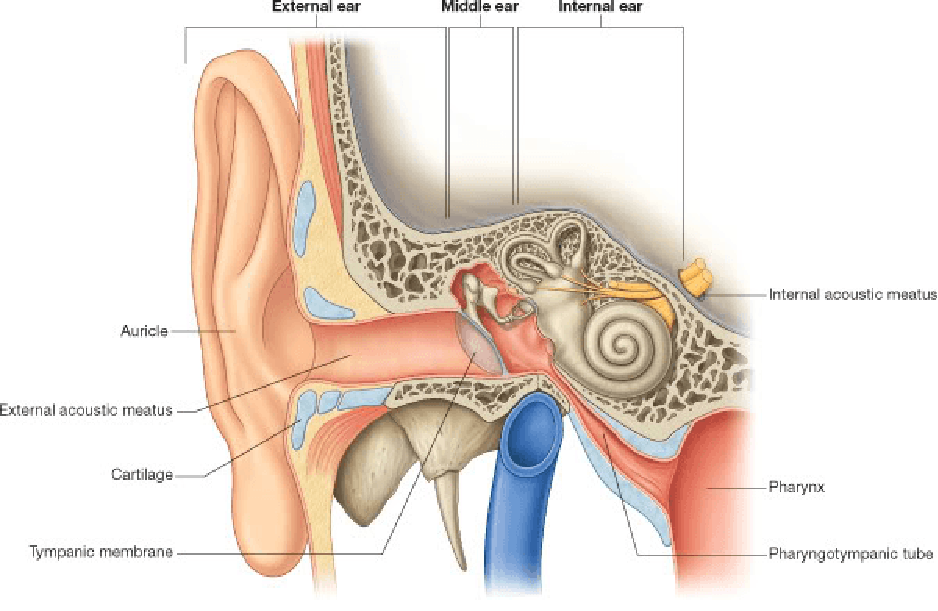
\includegraphics[scale=0.7]{figs/EarSection}
   \caption{Structure of the ear (Drake et al: Gray's Anatomy for Students)}
   \label{fig:EarSection}
\end{figure}
 
The ear canal in adults is approximately 25 mm long and have a diameter of 5 to 7 mm \citep{alvord1997anatomy}. The outer third of the external ear canal is surrounded by cartilage and fibrous tissue \citep{ExternalAuditoryCanal}. The inner two thirds are surrounded by the temporal bone. Thin skin from the lining of the canal and contains glands secreting ear wax. Hairs are found in the outer part of the canal. The ear canal of infants starts out relatively straight, but obtains a definite S-shape as the head develops \citep{alvord1997anatomy}. This S-shape is important to keep in mind while placing a sensor to measure tympanic temperature. Ear canal size also varies from person to person. Therefore, an ear probe should be designed to fit in a variety of in ear canal shapes and sizes.

\medskip
The secluded nature of the ear canal means that it has a relative constant temperature. Air trapped in the canal by a plug of high thermal resistance will reach thermal equilibrium close to the temperature of the canal wall and tympanum. This is a better location for a core temperature measurement, but will still be influenced by the ambient temperature.

\medskip
The wall of the ear canal is well supplied with blood. Blood vessels just beneath the thin layer of skin makes the ear canal a possible location for measuring heart rate and blood oxygen saturation. The still nature of the head will minimize movement artefacts.

\medskip
The ear canal extend toward the brain and electrical brain activity is present due to the conductive nature of the tissue. According to \cite{nunez2006electric} currents from brain potentials can be focused through holes in the scull, like the ear and nose. The farther away the origin of the signal is from the electrode, the weaker the measured signal will be. Therefore, an electrode in the ear canal will detect electrical brain activity near the ear better, including the temporal lobe and brain stem.

\subsection{Tympanic Membrane}
The tympanum forms the medial boundary of the external ear canal. It is a smooth elliptical membrane with a thickness of about 0.074 mm \citep{alvord1997anatomy}. The membrane is slanted with regards to the external ear canal.

\medskip
As with the rest of the external ear, the tympanum is supplied with blood from a branch of the carotid artery, therefore sharing its supply with the brain including the hypothalamus, the thermoregulation centre of the body. It is the most medial part of the external ear, and is therefore the least susceptible to influence by the ambient temperature. This is the reason that the tympanum is one of the best locations to measure core body temperature. The location is used by physicians to measure core temperature for it is quick and minimally invasive. Variations in body temp can be sensed faster on the tympanic membrane than on other locations on the body. Contact with the tympanum can cause discomfort and harm to the patient, so non-contact infra-red thermometers are usually used.


\section{Medical Sign Physiology} %----------------------------------------------------------------------------------
This section reviews the theory and research done about the physiological aspects of each medical sign that the Ear-Monitor is required to measure. The importance of each of the five medical signs will be discussed, including the typical range of measurements expected from healthy adults and the causes and implications of deviations from these healthy measurements.

\subsection{Core Temperature}
Thermoregulation is the body's way of keeping its internal temperature within certain bounds to create a favourable environment for chemical reactions to take place. The temperature control centre of the body is in the hypothalamus and it regulates temperature by maintaining a fine balance between heat production and heat loss. Normal human core temperature varies between $36.5^{\circ}C$ and $37.5^{\circ}C$ \citep{jones2010biomedical}. Inability to maintain this balance may indicate problems in the well-being of a person. Elevated temperature (hyperthermia) due to a fever can indicate the presents of an infectious disease. Abnormally low temperature (hypothermia) can be caused by cold exposure, metabolic disorders or infection. Both hyper- and hypothermia can be life threatening. A core temperature measurement is often a key indication to start a treatment or not. Therefore, temperature measurement is part of a full clinical examination and part of the vital sings group of medical signs.

\medskip
The location where temperature is measured is a key factor, for temperature is not constant throughout the body. This is because heat production and heat loss are not constant throughout the body, meaning extremities are usually cooler than the core. Traditional locations for measuring temperature are the tympanic membrane, axilla, mouth, rectum, oesophagus, forehead and urinary bladder. The mean temperature of these areas varies as well. A systematic literature review done by \cite{sund2002normal} combined the results of 20 studies to identify oral, rectal, tympanic and axillary temperature ranges in healthy humans. Table~\ref{fig:VariationsInTemp} shows the results.

 \begin{figure}
   \centering
   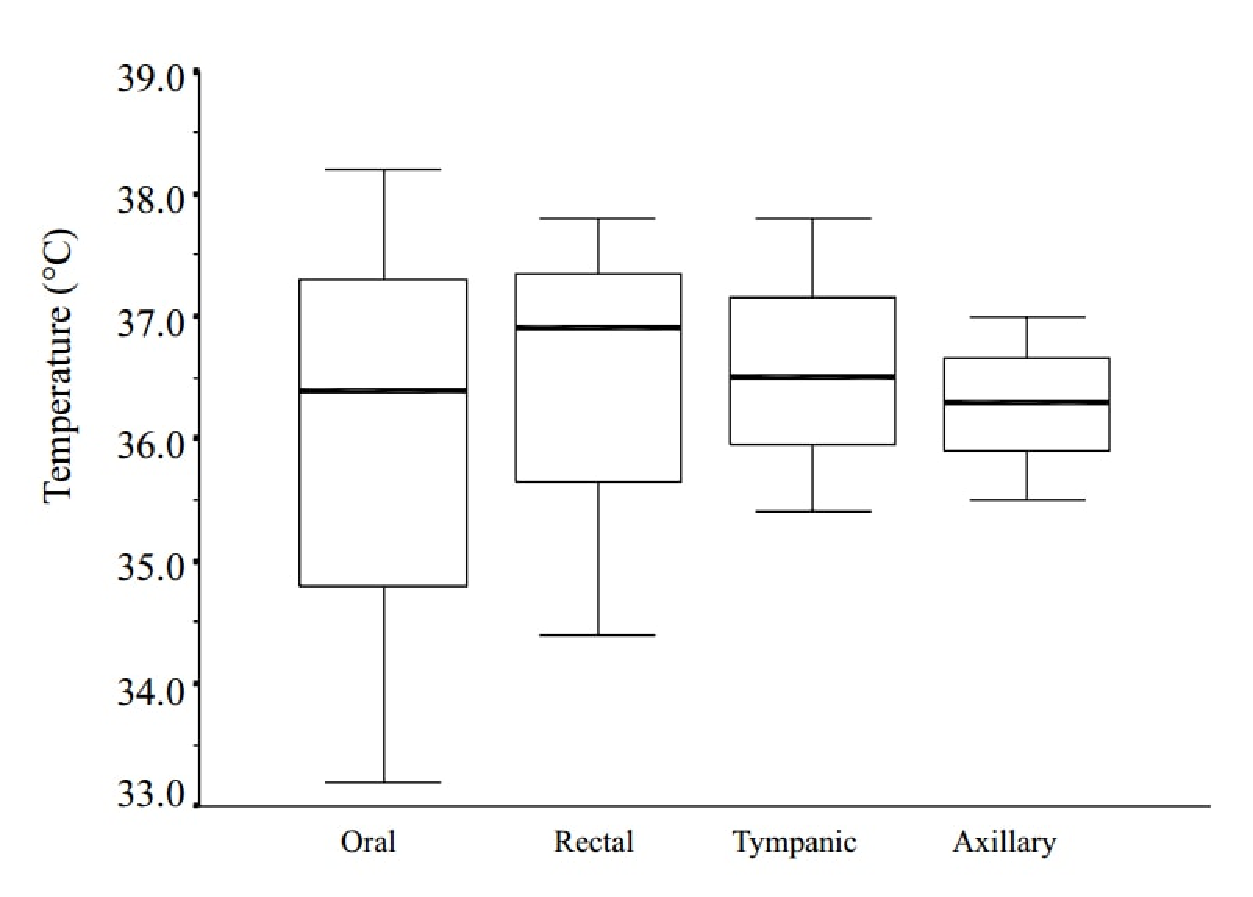
\includegraphics[scale=0.3]{figs/VariationsInTemp}
   \caption{The results from 20 studies with strong or fairly strong evidence of normal oral, rectal and tympanic temperature ($^{\circ}$C) in adult men and women are presented. Temperature is obtainable as mean value(bold lines), 1st and 3rd quartiles (unfilled bars) and range (thin lines).}
   \label{fig:VariationsInTemp}
\end{figure}





Studies have also been done comparing measurements at distinct locations to pulmonary artery temperature in ill patients. A study has shown ear-based  $0.07\pm 0.41$  $^{\circ}C$; urinary bladder  $0.03\pm 0.23^{\circ}C$; oral  $0.05\pm 0.26^{\circ}C$; and axillary $-0.68\pm 0.57 ^{\circ}C$. The accuracy of each method varied with the level of pulmonary artery temperature. Repeated measurements with all four methods had mean standard deviation values within $\pm 0.2^{\circ}C$ \citep{erickson1993comparison}.

\medskip
A second study done by \cite{lefrant2003temperature} showed the following results: oesophageal  $0.11 \pm 0.30^{\circ}C$, rectal $-0.07 \pm 0.40^{\circ}C$, axillary $0.27\pm 0.45^{\circ}C$, inguinal $0.17 \pm 0.48^{\circ}C$, urinary bladder $-0.21 \pm 0.20^{\circ}C$.

\medskip
The location of the device in development is restricted to the ear, therefore the tympanic membrane is the preferred location to take temperature measurements. The referenced studies show that the tympanic membrane is a valid location to measure accurate core temperature.

\subsection{Heart Rate}
The presence of a heart beat is paramount to sustain the vital cardiac output, supplying blood to the whole body. Heart rate can be controlled or maintained through two different regulatory systems: The intrinsic conduction system and the nervous system. The intrinsic conduction system works through the rhythmic contraction and relaxation of the heart muscle tissue. The heart rhythm is regulated by the sinoatrial node. The nervous system can influence the heart rate through sympathetic and parasympathetic nerves running from the cardiovascular centres in the medulla oblongata to the heart. The heart beat rate is varied to control the blood flow and blood pressure in the body.

\medskip
The heart is the source of a group of biosignals. The firing of nodes and propagation of electrical charges through neurons and the conductive cardiac muscle gives of an electrical signals that can be detected. The contraction of the  ventricles forces blood into the arteries, causing a temporary increase in blood pressure. This pressure increase propagates though the arteries as a wave, causing a temporary local increase on blood volume. Pressure- and volume changes can be detected. Blood turbulence and the opening and closing of heart valves causes the characteristic heart sound and chest movements, both indications of heart rate.

\medskip
Heart rate is influenced by numerous physiological factors including $O_2$, $CO_2$, $H^+$ levels, blood pressure, stress and exercise. Pathological factors can include fever, sepsis, heart disease and anaemia. Tachycardia is abnormally high resting heart rate, generally above 100 bpm, whereas bradycardia is a lower than normal resting heart rate, usually below 60 bpm \citep{normalRestingHR}. Although these two conditions are not necessarily danger signs, it may be an indication of health problems and therefore heart rate measurement is part of any medical examination and one of the vital signs group of medical signs.

\subsection{Respiratory Rate}
Respiration is the first step in the chain of events to get oxygen to the body's cells for metabolism to provide the body with energy. Respiration ventilates the lungs with air through inhalation and exhalation. The respiratory rate of a healthy adult at rest is usually between 12 and 20 breaths per minute \citep{medscapeBreathingRate}. This can vary drastically if the body is experiencing physical or emotional stress. In increase in respiratory rate can be cause by a fever, pulmonary dysfunction or any one of numerous medical conditions. Respiratory rate is also part of the vital signs group of medical signs.

\medskip
Respiratory rate monitoring is especially useful for diagnosing sleep apnoea. Symptoms include regular pauses in respiration or periods of shallow breathing (hypopnea) during sleep. This causes an oxygen deficiency in the body and lowers the quality of sleep. Short term symptoms include excessive daytime sleepiness, morning headaches, impaired alertness, and vision problems. If left untreated sleep apnoea can lead to high blood pressure, diabetes, depression, worsening of ADHD, stroke, heart failure, irregular heartbeats, and heart attacks \citep{webMDSleepApnoea}. Sufferers may be unaware of their condition and a sure-fire method of diagnosing it is my monitoring respirator rate during sleep, traditionally done during an overnight sleep study.

\subsection{Blood Oxygen Saturation}

Haemoglobin is the oxygen transporter protein found in the red blood cells of blood. Blood gets oxygenated in the lungs and then carries $O_2$ to the rest of the body for aerobic respiration necessary to produce energy. The correct levels of oxygen in the blood is vital to the health of the individual.

\medskip
Oxygen saturation, $SO_2$, refers to the concentration fraction of oxygenated haemoglobin to total concentration of haemoglobin in the blood:

$$SO_2  =  \frac{C(HbO_2)}{C(HbO_2)+C(Hb)}$$

Where $C(HbO_2)$ is the concentration of deoxygenated haemoglobin (deoxyhaemoglobin) and $C(Hb)$ is the concentration of oxygenated haemoglobin (oxyhaemoglobin).

\medskip
Blood oxygen saturation of 95-100\% is normal in healthy humans. Hypoxaemia is the condition when the saturation is below 90\%. This can be an indication of circulatory or ventilatory problems, anaemia or sleep apnoea. Levels below 80\% can hinder organ function and can lead to organ failure and cardiac- or respiratory arrest. The brain in extremely susceptible to damage due to a lack of oxygen. Cerebral hypoxia is the insufficient supply of oxygen to the brain. This can cause brain damage and in severe cases, brain death.

\subsection{Electrical Brain Activity}
EEG, or electroencephalography, is the non invasive recording of the electrical activity in the brain over time. The neurons in the brain conduce electrical current


\cite{bickford1951electroencephalography}

\begin{figure}[h]
\centering
\graphicspath{{figs/}}
\def\svgwidth{300pt}
\input{figs/eegRhythm.pdf_tex}
\caption{EEG rhythms}
\label{fig:eegRhythm}
\end{figure}
